\begin{enumerate}
	\item The digital circuit shown in Fig. \ref{fig:2004-gate-ee-68} generates a modified clockpulse at the output. Sketch the output waveform.
\label{prob:2004-gate-ee-68}
\hfill (GATE EE 2004)


\begin{figure}[h]
	\centering
	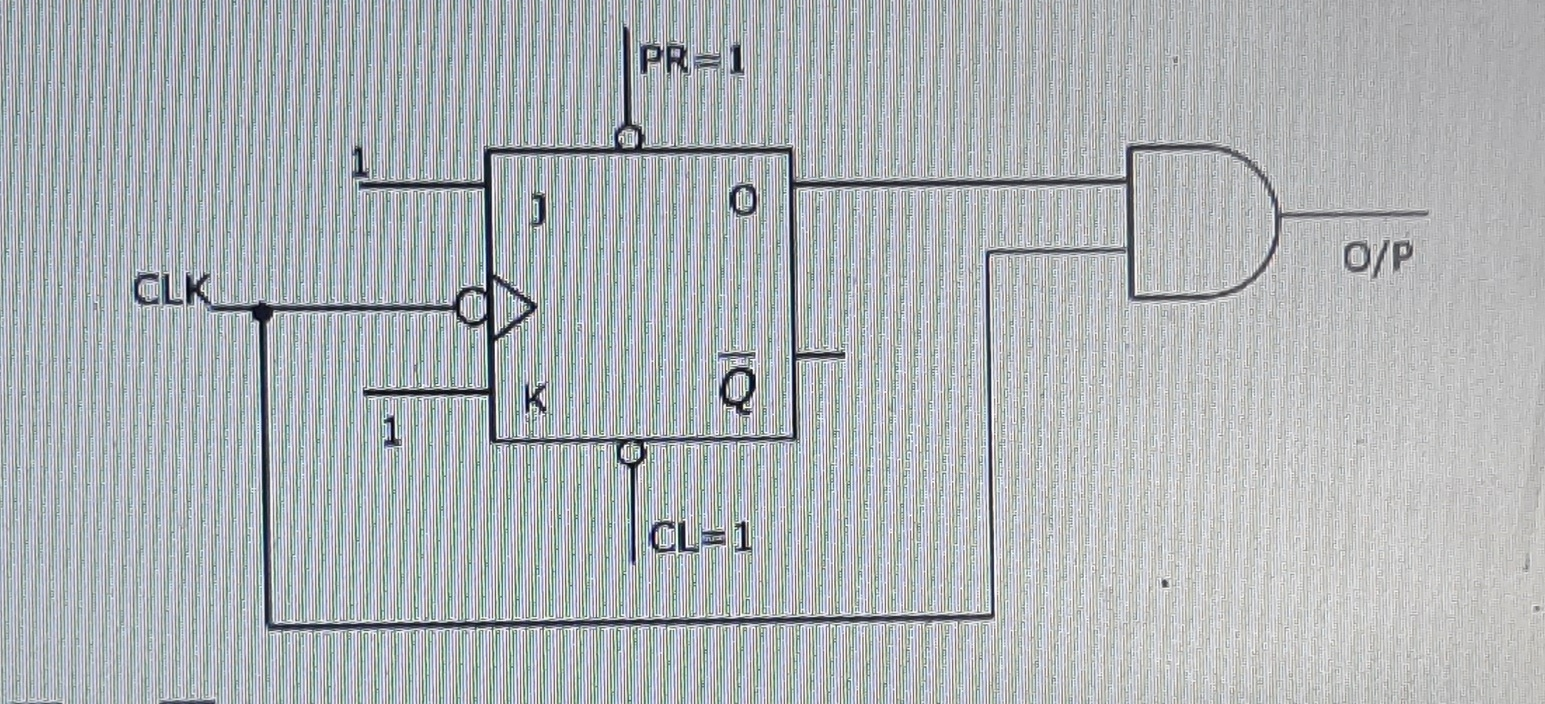
\includegraphics[width=\columnwidth]{figs/2004-gate-ee-68.jpg}
	\caption{}
\label{fig:2004-gate-ee-68}
\end{figure}
\item The circuit shown in the figure below uses ideal positive edge-triggered synchronous J-K flip flops with outputs X and Y. If the initial state of the output is X=0 and Y=0, just before the arrival of the first clock pulse, the state of the output just before the arrival of the second clock pulse is
\label{prob:2019-gate-in-12}
\hfill (GATE IN 2019)
\begin{figure}[!h]
	\begin{center} 
	    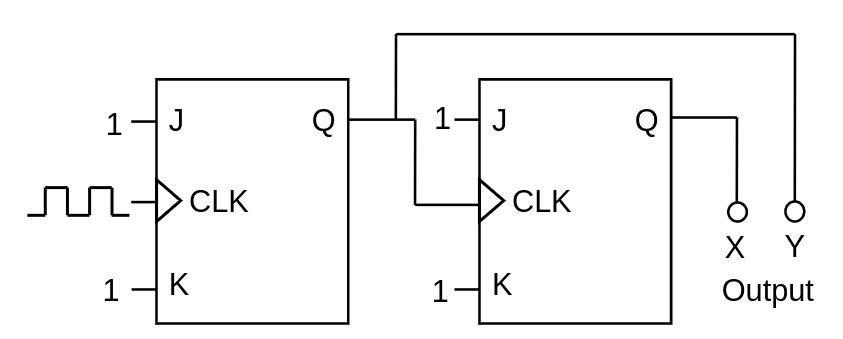
\includegraphics[width=\columnwidth]{figs/2019-gate-in-12.png}
	\end{center}
\caption{}
\label{fig:2019-gate-in-12}
\end{figure}
\item 	The state diagram of a sequence detector is shown in
  \figref{fig:gate/ec/2020/39/1}		
		. State $S_0$ is the initial state of the sequence detector. If the output is 1, then
\hfill (GATE EC 2020)
 \begin{figure}[h]
	 \centering
  \begin{tikzpicture} [node distance=2cm]
\centering 
\node[circle, draw, state, initial] (S0) {$S_0$};
\node[circle, draw, state, accepting, right of=S0] (S1) {$S_1$};
\node[circle, draw, state, accepting, right of=S1] (S2) {$S_2$};
\node[circle, draw, state, accepting, right of=S2] (S3) {$S_3$}; 
\node[circle, draw, state, below right of = S1] (S4) {$S_4$};
\path[->] (S0) edge[above] node{0/0} (S1) 
          (S0) edge[loop above] node{1/0} (S0)
          (S1) edge[above] node{1/0} (S2)
          (S1) edge[loop above] node{0/0} (S1)
          (S2) edge[above] node{0/0} (S3) 
          (S2) edge[below,bend left] node{1/0} (S0)
          (S3) edge[below] node{1/0} (S4) 
          (S3) edge[above,bend right] node{0/0} (S1) 
          (S4) edge[below,bend left] node{1/0} (S0)   
          (S4) edge[below,bend right] node{0/1} (S3); 
\end{tikzpicture}

  \caption{State diagram}
  \label{fig:gate/ec/2020/39/1}		
  \end{figure}	 
\begin{enumerate}
 \item the sequence 01010 is detected
 \item the sequence 01011 is detected
 \item the sequence 01110 is detected
 \item the sequence 01001 is detected	 
\end{enumerate}	
	\item 		
		A counter is constructed with three D flip-flops. The input-output pairs are named (D0, Q0), (D1, Q1), and (D2, Q2), where the subscript 0 denotes the least significant bit. The output sequence is desired to be the Gray-code sequence 000, 001, 011, 010, 110, 111, 101, and 100, repeating periodically. Note that the bits are listed in the Q2 Q1 Q0 format. Find the combinational logic expression for D1.
\label{prob:2021-gate-ee-37}
\hfill (GATE EE 2021)
\iffalse
\item The propogation delay of the exclusive-OR(XOR) gate in the circuit in Fig.
\label{prob:2021-gate-ec-46}
\ref{fig:2021-gate-ec-46}
is 3ns. The propogation delay of all the flip-flops is assumed to be zero. The clock(Clk) frequency provided to the circuit is 500MHz.
\begin{figure}[!h]
\begin{center}
\resizebox{0.5\columnwidth}{!}{
\begin{tikzpicture}
\ctikzset{                                   
logic ports=ieee,                   
logic ports/scale=0.5               
}                                    
\draw(-1.3,0)node[xor port,anchor=out](x) {};         
\tikzstyle{dff}=[rectangle,draw,minimum height=7em,text width=7em,inner sep=3em]                                       
\node[dff] (dff2) {D2};                             
\node[dff, right=2cm of dff2] (dff1) {D1};           
\node[dff, right=2cm of dff1] (dff0) {D0};        
%Connecting flip-flops together                    
\draw (dff2.out) -- ++(2,0) node[above]{};        
\draw (dff1.out) -- ++(2,0) node[above] {};         
\draw (dff0.out) -- ++(2,0) node[above]{};          
\draw(dff2.out) -| (2.3,1.5) node[above]{$Q2$};        
\draw(dff1.out) -|(6.8,1.2) node[above]{$Q1$};         
\draw(dff0.out) -|(12.4,2) node[above]{$Q0$};          
\draw(x.in 2) -|(-3,2)to[short] (12.4,2);              
\draw(x.in 1)-|(-2.5,1.5)to[short](2.3,1.5);          
\draw(-2,-2) node[above]{$Clk$} --(6,-2);            
\draw(6,-2) node[above]{} --(9.1,-2);                 
\draw(9.1,-2)--(9.1,-1.2) node[above]{};                 
\draw(8.9,-1.23)--(9.1,-1)--(9.3,-1.23);               
\draw(4.5,-2)--(4.5,-1.2) node[above]{};               
\draw(4.3,-1.23)--(4.5,-1)--(4.7,-1.23);            
\draw(0,-2)--(0,-1.2) node[above]{};               
\draw(-0.2,-1.23)--(0,-1)--(0.2,-1.23);
\end{tikzpicture}

}
\end{center}
	\caption{Circuit}
\label{fig:2021-gate-ec-46}
\end{figure}
%
Starting from the initial value of the flip-flop outputs $Q2Q1Q0 =111$ with $D2=1$,the minimum number of triggering clock edges after which the flip-flop outputs $Q2Q1Q0$ becomes 1 0 0\emph{(in integer)} is \line(1,0){12.5}
\hfill (GATE EC 2021)
\fi
\item 
\label{prob:2022-gate-ec-43}
	 For the circuit shown in Fig. 
\ref{fig:2022-gate-ec-43},
		the clock frequency is $f_0$ and the duty cycle is $25 \%$. For the signal at the $Q$ output of the Flip-Flop,
\begin{enumerate}
	\item frequency of $\frac{f_0}{4}$ and duty cycle is 50$\%$
	\item frequency of $\frac{f_0}{4}$ and duty cycle is 25$\%$
	\item frequency of $\frac{f_0}{2}$ and duty cycle is 50$\%$
	\item frequency of $f_0$ and duty cycle is 25$\%$ \\
\end{enumerate}
\begin{figure}[h]
	\centering
\begin{tikzpicture}
    \draw (2,2) rectangle (5,5);
    \draw (3.5,5) node[above]{$2$ $Bit$ $binary$ $counter$};
    \draw (3.3,2) -- (3.5,2.2) -- (3.7,2);
    \draw (7,2) rectangle (10,5);
    \draw (8.5,5) node[above]{$Flip-Flop$};
    \draw (8.3,2) -- (8.5,2.2) -- (8.7,2);
    \draw (5,3) -- (5.5,3) node[above]{$MSB$} -- (6,3);
    \draw (7.25,3) node{$K$};
    \draw (5,4) -- (5.5,4) node[above]{$LSB$} -- (7,4);
    \draw (7.25,4) node{$J$};
    \draw (6.75,4) -- (6.75,3) -- (7,3);
    \draw (0,0) node[above]{$clock$} -- (8.5,0);
    \draw (3.5,0) -- (3.5,2);
    \draw (8.5,0) -- (8.5,2);
    \draw (10,3) -- (11,3);
    \draw (9.75,4) node{$Q$} (10,4) -- (11,4);
\end{tikzpicture}

	\caption{}
\label{fig:2022-gate-ec-43}
\end{figure}
\hfill 	(GATE EC-2022)

\item A sequence detector is designed to detect precisely 3 digital inputs, with overlapping sequences detectable. For the sequence $(1,0,1)$ and input data $(1,1,0,1,0,0,1,1,0,1,0,1,1,0)$, what is the output of this detector?
		\begin{enumerate}
			\item 1,1,0,0,0,0,1,1,0,1,0,0
			\item 0,1,0,0,0,0,0,1,0,1,0,0
			\item 0,1,0,0,0,0,0,1,0,1,1,0
			\item 0,1,0,0,0,0,0,0,1,0,0,0
		\end{enumerate}
		\hfill (GATE EE 2020)
\item 
 Two T-flip flops are interconnected as shown in \figref{fig:tff1}. The present state of the flip flops are: $A = 1, B = 1$. The input x is given as $1, 0, 1$ in the next three clock cycles. The decimal equivalent of $(ABy)_{2}$ with A being the MSB and y being the LSB, after the 3\textsuperscript{rd} clock cycle is \rule{12mm}{0.4pt}

		\vspace{1cm}
	\begin{figure}[ht]
		\centering
		\begin{tikzpicture}
  \draw (0,0) rectangle (2,3);

  \draw (-4,2.25) -- (0,2.25);
  \draw (-0.5,0.75) -- (0,0.75);
  \node[left] at (0.75,2.25) {$T_B$};
  \node[left] at (1.1,0.75) {$clk$};

  \draw (2,2.25) -- (4,2.25);
  \node[left] at (2,2.25) {$B$};
  

  \draw (0,0.4) -- (0.4,0.75) -- (0,1.1);

  \draw (0,4) rectangle (2,7);
  
  \draw (-0.5,6.25) -- (0,6.25);
  \draw (-0.5,4.75) -- (0,4.75);
  \node[left] at (0.75,6.25) {$T_A$};
  \node[left] at (1.1,4.75) {$clk$};

  \draw (-1.5,6.25) node[nand port] (nand) {};
  \draw (-4.5,6.525) -- (nand.in 1);
  \node[left] at (-4.5,6.525) {$x$};
  \draw (-2.9,3.5) -- (nand.in 2) ;
  \draw (nand.out) -- (-0.5,6.25) ;
  \draw (-4,2.25) -- (-4,6.525) ;
  \draw (-2.9,3.5) -- (3.5,3.5) ;
  \draw (3.5,3.5) -- (3.5,2.25) ;
  \filldraw (3.5,2.25) circle (2pt) ;
  \filldraw (-4,6.525) circle (2pt) ;
  \filldraw (-0.5,0.75) circle (2pt);

  \draw (5.5,5.965) node[or port] (or) {};
  \draw (4,6.25) -- (or.in 1) ;
  \draw (4,2.25) -- (4,5.685) ;
  \draw (4,5.685) -- (or.in 2) ;
  \node[right] at (or.out) {$y$} ;
  \draw (-0.5,4.75) -- (-0.5,-1.) ;
  \node[below] at (-0.5,-1.) {$clk$};
  
  \draw (2,6.25) -- (4,6.25);
  \node[left] at (2,6.25) {$A$};

  \draw (0,4.4) -- (0.4,4.75) -- (0,5.1);
  
\end{tikzpicture}
		\caption{}
		\label{fig:tff1}
		\hfill (GATE IN 2020)
	\end{figure}


\item In the circuit shown below,\ref{fig:image} a positive edge-triggered D flip-flop is used for sampling input data
 using clock CK.The XOR gate outputs 3.3 volts for logic HIGH and 0 volts for logic LOW levels.
The data bit and clock periods are equal and the value of $ \Delta T / T_{ck} $ = 0.15,where
the parameters $ \Delta T $ and $ T_ck$ are shown in the figure.Assume  that the Flip and
the XOR gate are ideal.  
\begin{figure}[!ht] 
    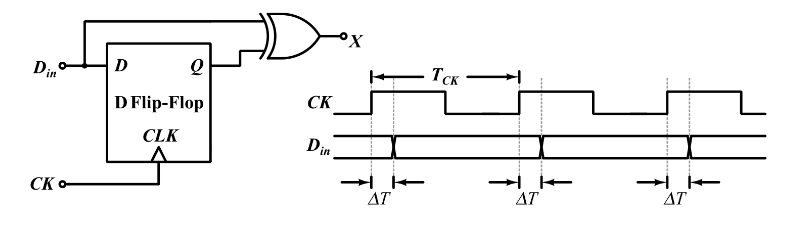
\includegraphics[scale=0.4]{figs/image.png} 
    \caption{image}
    \label{fig:image}
 \end{figure}
\label{fig:2018-gate-ec-46}
\hfill(GATE EC 2018)
\item A 2-bit synchronous counter using two J-K flip flops is shown. The expressions for the inputs to the J-K flip flops are also shown in the figure. The output sequence of the counter starting from $Q_1Q_2 = 00$ is 
\begin{figure}[!ht]
	\centering
	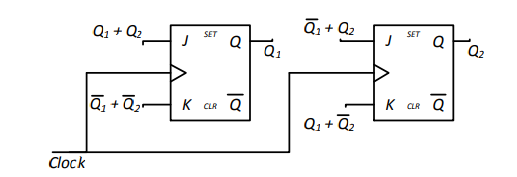
\includegraphics[width=\columnwidth]{figs/question44.png}
	\caption{$2$-bit synchronous counter}
	\label{fig:enter-label}
\end{figure}
\begin{enumerate}
	\item $00\rightarrow11\rightarrow10\rightarrow01\rightarrow00...$ 
        \item $00\rightarrow01\rightarrow10\rightarrow11\rightarrow00...$
        \item $00\rightarrow01\rightarrow11\rightarrow10\rightarrow00...$
        \item $00\rightarrow10\rightarrow11\rightarrow01\rightarrow00...$
\end{enumerate}
\hfill{GATE IN 2018}
        \item Let $p$ and $q$ be two propositions. Consider the following two formulae in propositional logic.
			\begin{align}
				 S_1 : ( \rightharpoondown p \vee (p \wedge q))\rightarrow q \\
				 S_2 : q\rightarrow(\rightharpoondown p \vee (p \wedge q))
			\end{align}
        Which one of the following choices is correct?
		                                          \hfill(GATE-CS2021)
		\begin{enumerate}[label=(\Alph*)]
			\item Both $S_1$ and $S_2$ are tautologies.
			\item $S_1$ is a tautology but $S_2$ is not a tautology.
			\item $S_1$ is not a tautology but $S_2$ is a tautology.
			\item Neither $S_1$ nor $S_2$ is a tautology.
		\end{enumerate}
\item Consider a $3$-bit counter, designed using T flip-flops, as shown below:
     \begin{figure}[H]
\centering
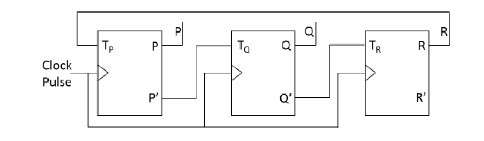
\includegraphics[width=\columnwidth]{ide/fsm/figs/3bitcounter.jpg}
\caption{}
\label{fig:3bitcounter.jpg}
\end{figure}
Assuming the initial state of the counter given by $PQR$ as $000$,what are the next three states?
                 \hfill(GATE-CS2021)
\begin{enumerate}[label=(\Alph*)]
\item $011, 101, 000$
\item $010, 101, 000$
\item $010, 101, 000$
\item $010, 101, 000$
\end{enumerate}

\item The state diagram of a sequence detector is shown below. state S0 is the initial state of the sequence detector. If the output is 1,then
                                        \hfill(GATE-EC2020,39)
\begin{figure}[H]
    \centering
    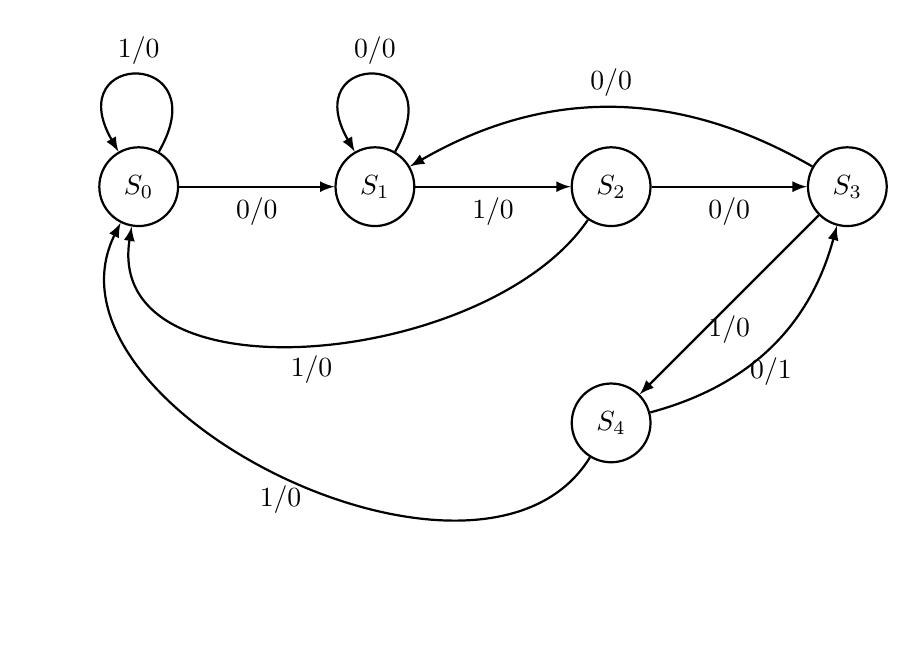
\begin{tikzpicture}[-latex ,node distance=3cm and 1cm,thick,state/.style={circle ,draw, minimum width =1cm}]
  \node[state] (S0) {$S_0$};
  \node[state] (S1) [right of=S0] {$S_1$};
  \node[state] (S2) [right of=S1] {$S_2$};
  \node[state] (S3) [right of=S2] {$S_3$};
  \node[state] (S4) [below of=S2] {$S_4$};

\path (S0) edge [loop above ,out=60, in=120, distance=1.5cm] node {1/0} (S0)
      (S2) edge [bend left , out=55, in=80] node [below=0.15] {1/0} (S0)
      (S1) edge [loop above ,out=60, in=120, distance=1.5cm] node {0/0} (S1)
      (S0)  edge node [below=0.15] {0/0} (S1)
      (S1) edge node [below=0.15] {1/0} (S2)
      (S2) edge  node [below=0.15] {0/0} (S3)
        (S3) edge [bend right] node[above=0.15] {0/0} (S1)
        (S4) edge [bend right] node [below=0.25] {0/1} (S3)
        (S4) edge [bend left=-40 , out=85, in=90] node [below=0.15] {1/0} (S0)
           (S3) edge node [below=0.15] {1/0} (S4);
\end{tikzpicture}


    \caption{State diagram of a sequence detector}
     \label{fig:enter-label}	
\end{figure}
\begin{enumerate}
\item   the sequence $01010$ is detected.
\item   the sequence $01011$ is detected.
\item   the sequence $01110$ is detected.
\item   the sequence $01001$ is detected.
\end{enumerate}


\item The state transition diagram for the circuit shown is
                         \hfill(GATE-IN2019,39)
\begin{figure}[H]
\centering
\begin{circuitikz}
            \draw (2,2)coordinate(w)--(5,2)coordinate(x)--(5,6)coordinate(x)--(2,6)coordinate(z)--(2,2)coordinate(w);
            \draw (0.85,5.5)--(2,5.5);
            \draw (2,5.5)node[right]{$D$};
            \draw (1,0)--(1,2.5)--(2,2.5);
            \draw (1,-0.5)node[]{$CLK$};
            \draw (2,2.25)--(2.3,2.5)--(2,2.75);
            \draw (5,5.5)node[left]{$Q$}--(8,5.5)node[right]{$1$};
            \draw (5,2.5)node[left]{$\overline{Q}$}--(8,2.5)node[right]{$0$};
              % Reversed NAND gate (horizontally flipped)
    \draw (5,8) node[nand port,scale=-1] (nand) {};
    %\draw (nand.in 1) node[left] {};
%\draw (nand.in 2) node[left] {};
    
    % Output
    
    \draw (nand.out) -- ++(-4,0) -- ++(0,-2.5) node[above]{};
    % Inputs
    \draw (nand.in 1) -- ++(0,-2.2) node[below]{};
    \draw (nand.in 2) -- ++(4,0)--++(0,-4.2)--++(-0.86,0) node[below]{};
    \draw (8,2)--(8,6)--(9.5,5)--(9.5,3)--(8,2);
    \draw [->](9,0)node[right]{$A$}--(9,2.7);
    
\end{circuitikz}

\caption{Circuit~Diagram}
\end{figure}

\begin{enumerate}
%% options1
\item 
\begin{figure}[H]
\centering
\begin{circuitikz}
[-latex ,node distance=4cm and 2cm,thick,state/.style={circle,draw, minimum width =1cm}] 

\node[state] (Q0) {$Q=0$};
\node[state] (Q1) [right of=Q0]{$Q=1$};
\path (Q0) edge [bend left] node [above=0.15] {A = 1} (Q1);
\path (Q0) edge [loop above ,out=100 ,in=150,distance=2cm] node {A = 0} (Q0);
\path  (Q1) edge [bend left] node [below=0.15] {A = 1} (Q0);
\path (Q1) edge [loop above ,in=60,out=120,distance=2cm] node {A=0} (Q1);
        
\end{circuitikz}


\end{figure}
%% options2
\item \begin{figure}[H]
\centering
\begin{circuitikz}[-latex ,node distance=4cm and 2cm,thick,state/.style={circle,draw, minimum width =1cm}]
\node[state] (Q0) {$Q=0$};
\node[state] (Q1) [right of=Q0]{$Q=1$};
\path (Q0) edge [bend left] node [above=0.15] {A = 1} (Q1);
\path  (Q1) edge [bend left] node [above=0.15] {A = 1} (Q0);
\path (Q0) edge [loop above ,out=100,in=150,distance=2cm] node {A = 0} (Q0);
\path (Q1) edge [bend left ,out=85,in=90] node [above=0.15] {A = 0} (Q0);
\end{circuitikz}


\end{figure}
%% options3
\item 
\begin{figure}[H]
\centering
\begin{circuitikz}
[-latex ,node distance=4cm and 2cm,thick,state/.style={circle,draw, minimum width =1cm}]

\node[state] (Q0) {$Q=0$};
\node[state] (Q1) [right of=Q0]{$Q=1$};
\path (Q0) edge [bend left] node [above=0.15] {A = 1} (Q1);
\path  (Q1) edge [bend left] node [above=0.15] {A = 1} (Q0);
\path (Q1) edge [loop above ,in=20,out=70,distance=2cm] node {A = 0} (Q1);
\path (Q0) edge [bend left ,out=85,in=90] node [above=0.15] {A = 0} (Q1);  
\end{circuitikz}


\end{figure}
%% options4
\item 
\begin{figure}[H]
\centering
\begin{circuitikz}[-latex ,node distance=4cm and 2cm,thick,state/.style={circle,draw, minimum width =1cm}]
\node[state] (Q0) {$Q=0$};
\node[state] (Q1) [right of=Q0]{$Q=1$};
\path (Q0) edge [bend left] node [above=0.15] {A = 0} (Q1);
\path (Q0) edge [loop above ,out=100 ,in=150,distance=2cm] node {A = 1} (Q0);
\path  (Q1) edge [bend left] node [below=0.15] {A = 1} (Q0);
\path (Q1) edge [loop above ,in=60,out=120,distance=2cm] node {A=0} (Q1);
\end{circuitikz}


\end{figure}

\end{enumerate}

\end{enumerate}
\end{document}






\end{enumerate}

